\begin{titlepage}
  \begin{center}

  % Upper part of the page. The '~' is needed because \\
  % only works if a paragraph has started.
  %\includegraphics[width=0.15\textwidth]{./logo}~\\[1cm]

  \textsc{\LARGE Vyšší odborná škola a Střední průmyslová škola elektrotechnická Olomouc}%\\[1.5cm]

	% logo školy
	\begin{figure}[H]
    \centering
    \includegraphics[width=4cm]{img/logo/logo.pdf}
  \end{figure}

  \textsc{\Large SOUTĚŽ DĚTÍ A MLÁDEŽE V RADIOELEKTRONICE}\\[0.5cm]
  kategorie mládež\\[.2cm]
	
	
	
  % Title
  \HRule \\[0.4cm]
  { \huge \bfseries SDR přijímač pro pásmo KV\\[0.4cm] }

  \HRule \\[.5cm]
  
  SDR RECEIVER FOR SW BAND\\[1.5cm]
		
  % Author and supervisor
  \emph{Autor:} Jan \textsc{Vykydal}
  
  \vfill

  % Bottom of the page
  {\large \today}

  \end{center}
\end{titlepage}
